
\documentclass[tikz]{standalone}
\usepackage{tikz-3dplot}
\begin{document}
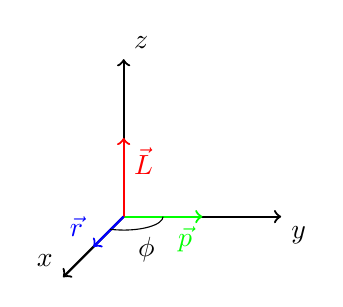
\begin{tikzpicture}
\tdplotsetmaincoords{70}{110}
\draw (0,0,0) node[above left] {};
\draw[thick, ->] (0,0,0) -- (2,0,0) node[anchor=north west]{$y$};
\draw[thick, ->] (0,0,0) -- (0,2,0) node[anchor=south west]{$z$};
\draw[thick, ->] (0,0,0) -- (0,0,2) node[anchor=south east]{$x$};

\draw[thick, ->,green] (0,0,0) -- (1,0,0) node[anchor=north east]
{$\vec{p}$};
\draw[thick, ->,red] (0,0,0) -- (0,1,0) node[anchor=north west]{$\vec{L}$};
\draw[thick, ->,blue] (0,0,0) -- (0,0,1) node[anchor=south east]{$\vec{r}$};
\tdplotdrawarc{(0,0,0)}{0.5}{0}{110}{anchor=north}{$\phi$}
\end{tikzpicture}
\end{document}